\newcommand{\usecase}[7]{
\begin{center}
\begin{tabular}[h!]{| l | p{13cm} |}
	\hline
	\textbf{Name} & #1 \\ \hline
	\textbf{Actors} & #2 \\ \hline
	\textbf{Goal} & #3 \\ \hline
	\textbf{Preconditions} & #4 \\ \hline
	\textbf{Basic Flow} & #5 \\ \hline
	\textbf{Alternative Flow} & #6 \\ \hline
	\textbf{Postconditions} & #7 \\ \hline
\end{tabular}
\end{center}
}

\section{Use Case Diagram}

\begin{center}
	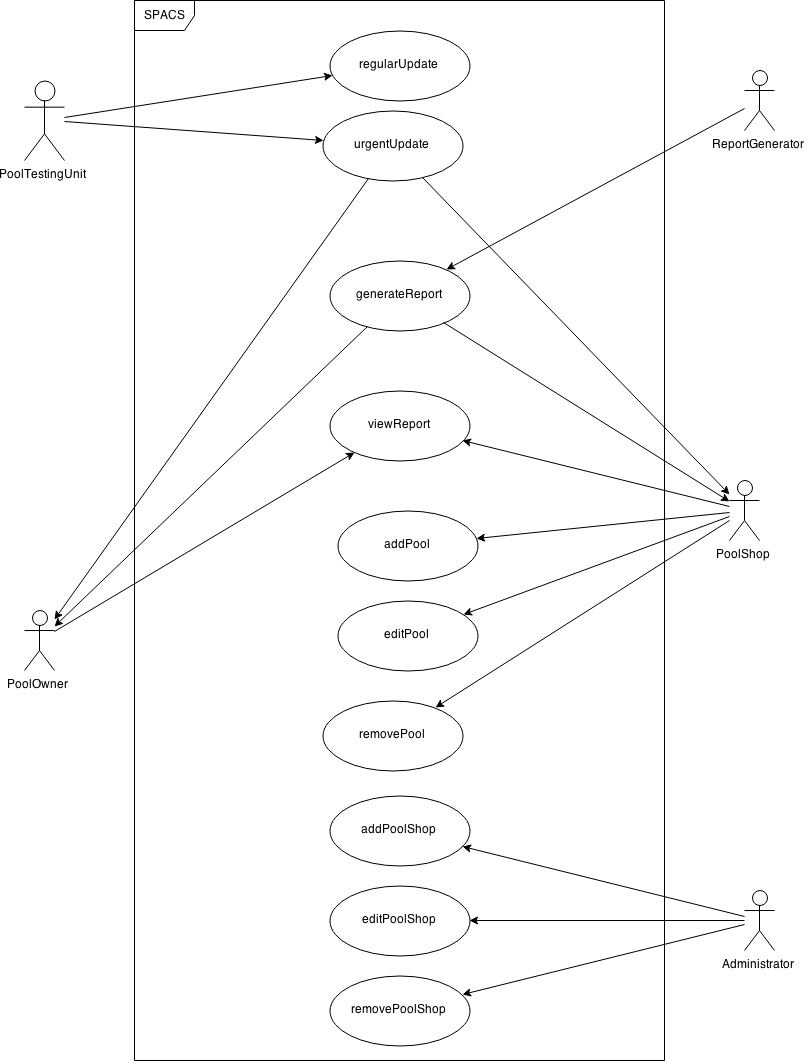
\includegraphics[width=15cm]{images/UseCaseDiagram}
\end{center}

\usecase
{regularUpdate}
{PoolTestingUnit}
{store collected information from the PTU in the system}
{PoolTestingUnit is authenticated}
{
\begin{enumerate}
\item Use case starts when ptu sends data
\item validate data
\item store it so that it can be used later
\item The use case ends
\end{enumerate}
}
{
\begin{enumerate}
\item Data is malformed
\begin{enumerate}
\item Recieved data is logged for analysis
\end{enumerate}
\item Issue storing data
\begin{enumerate}
\item Fall back to logging data and alert the administrator
\end{enumerate}
\end{enumerate}
}
{\begin{enumerate}
\item Success: Data has been stored
\item Failure: Data has been stored in a log for analysis by admin
\end{enumerate}}

\usecase
{urgentUpdate}
{PoolTestingUnit, PoolShopAdministrator, PoolOwner}
{store collected information from the PTU in the system and alert the pool owner and pool shop that there is a problem}
{PoolTestingUnit is authenticated}
{  - use case starts when ptu sends data with alerts
  - validate data
  - store it so that it can be used later
  - email is sent to the PoolShopOwner and PoolOwner
  - the use case ends}
{  - Data is malformed
    - Recieved data is logged for analysis
  - Issue storing data
    - Fall back to logging data and alert the administrator
  - Email fails
    - Email gets retried and event is logged}
{  Success: Data has been stored, email has been sent to PoolShopOwner and PoolOwner
  Failure: Data has been stored in a log for analysis by admin}

\usecase
{generateReport}
{PoolOwner, PoolShopAdministrator}
{provide latest data to }
{First week of the PTU or a month since the last report}
{  - use case starts at the same time every day
  - gets a list of pools that need reports
  - for each pool
    - gets the information that should be on the report
    - generates the report as a pdf
    - emails it off}
{}
{  Success: Report generated and emailed to pool owner and pool shop
  Failure: Any errors logged for admin to look over}

\usecase
{addPoolShop}
{Administrator}
{To add a pool shop to the system.}
{}
{  - Administrative user enters information about the pool shop}
{  - Invalid Information
    - Error displayed and user is able to re-enter}
{Success: Data is stored and can be retieved later
Failure: User is given achance to modify data}

\usecase
{editPoolShop}
{Administrator}
{To edit a pool shop in the system.}
{}
{  - Administrative user enters updated information about the pool shop}
{  - Invalid Information
    - Error displayed and user is able to re-enter}
{Success: Data is stored and can be retieved later
Failure: User is given achance to modify data}

\usecase
{removePoolShop}
{Administrator}
{To remove a pool shop from the system.}
{}
{  - Administrative selects the pool shop
  - Confirms that the pool shop should be disabled}
{  - Cancelled
    - No change is made}
{Data is no longer accessible. User no longer able to log in}
{No change}

\usecase
{addPool}
{PoolShopAdministrator}
{To add a pool to the system.}
{}
{}
{}
{}

\usecase
{editPool}
{PoolShopAdministrator}
{To edit a pool in the system.}
{}
{}
{}
{}

\usecase
{removePool}
{PoolShopAdministrator}
{To remove a pool from the system.}
{}
{}
{}
{}




